\subsection{M\'etodo CFD-DEM} \label{MCFDEM}

\noindent
\justify

En el acoplamiento cl\'asico entre CFD-DEM, el flujo se resuelve a trav\'e del m\'etodo CFD basado en malla, mientras que la fase s\'olida es modelada mediante DEM para cada part\'icula sujeta a trav\'es de fuerzas hidrodin\'amicas, fuerzas de cuerpo (como la gravedad) y a trav\'es de fuerzas de contacto, actualizando valores de velocidad y posici\'on conforme a la segunda ley de Newton (Hoomans \textit{et al.}, 1996; Tsuji \textit{et al.}, 1993; Xu y Yu, 1997). En principio, todos los m\'etodos CFD pueden acoplarse con DEM; lo que ha dado origen a diferentes m\'etodos discretos y continuos, tal como el m\'etodo de Lattice Boltzmann (LBM), Hidrodin\'amica de Part\'iculas Suaves (SPH), m\'etodos de Diferencias Finitas y Vol\'umenes Finitos (FVM).

\noindent
\justify

Gran parte de las simulaciones reportadas en la literatura comprenden modelos 2D o sistemas prototipados de peque\~na escala. En busca de acelerar los tiempos de simulaci\'on e incrementar la eficiencia computacional, se han desarrollado t\'ecnicas de computaci\'on paralela; donde gran parte de los esfuerzos han sido enfocados en la paralelizaci\'on del DEM. Muchos algoritmos se han propuesto para lograr este hecho, como la t\'ecnica de espejo de dominio (Damana, \textit{et al.}, 2006; Washington y Meegoda, 2003), el m\'etodo de subconjunto de part\'iculas (Kafui \textit{et al.}, 2011) y m\'etodos de descomposici\'on de dominios (Amritkar \textit{et al.}, 2014; Tsuji \textit{et al.}, 2008). El uso de estos algoritmos depende de la arquitectura del hardware. La paralelizaci\'on sobre memoria compartida del sistema se alcanza, normalmente, empleando \textit{OpenMP} (``Open Multi-Processing", por sus siglas en ingl\'es), mientras que el MPI (Interfaz de Paso de Mensajes) se emplea en sistemas de memoria distirbuida (Rabenseifner \textit{et al.}, 2009). Por ejemplo, Tsuji \textit{et al.} (2008) paralelizaron una simulaci\'on en CFD-DEM usando MPI para el intercambio de informaci\'on entre 16 CPUs, reportando el comportamiento fluidodin\'amico de 4.5 millones de part\'iculas en un medio gaseoso; empleando el m\'etodo unidimensional de descomposici\'on de dominio.

\subsubsection{Fase del solvente}

\noindent
\justify

En un modelo CFD-DEM, la fase del fluido se resuleve en el nivel computacional en cada elemento de la malla (ver Figura \ref{elemento}) empleando un marco de referencia Euleriano mientras que el movimiento de la part\'icula se sigue a trav\'es de un marco de referencia Lagrangiano. Para lograr el acoplamiento de fase, es necesario interpolar las propiedades de las part\'iculas a los centroides de los elementod CFD y las propiedades del fluido a la posici\'on de cada part\'icula. Como se muestra en la Figura \ref{particle}, se crean dos mallas alineadas de b\'usqueda: la malla de b\'usqueda de part\'iculas (amarilla) y la malla de b\'usqueda de fluido (azul). 

\begin{figure}[h!]
	\centering
	\begin{subfigure}[b]{0.3\textwidth}
		\centering
		\begin{adjustbox}{max width = \textwidth}
		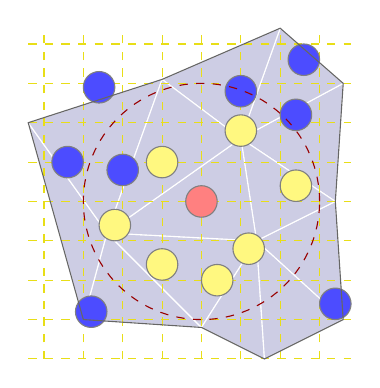
\begin{tikzpicture}
		%---Interno---
	%1 - (-1.2, -0.4)
	\draw[white, fill=blue!30!gray!30!white] (-1.5, -1.5) -- (0,-1.6) -- (-1.2, -0.4) -- cycle;
	\draw[white, fill=blue!30!gray!30!white] (-2.2, 1) -- (-1.5,-1.5) -- (-1.2, -0.4) -- cycle;
	\draw[white, fill=blue!30!gray!30!white] (-2.2, 1) -- (-0.5, 1.55) -- (-1.2, -0.4) -- cycle;
	%2 - (0.7, -0.5)
	\draw[white, fill=blue!30!gray!30!white] (-1.2, -0.4) -- (0,-1.6) -- (0.7, -0.5) -- cycle;
	\draw[white, fill=blue!30!gray!30!white] (0.8,-2) -- (0,-1.6) -- (0.7, -0.5) -- cycle;
	\draw[white, fill=blue!30!gray!30!white] (1.8,-1.5) -- (0.8,-2) -- (0.7, -0.5) -- cycle;
	\draw[white, fill=blue!30!gray!30!white] (1.8,-1.5) -- (1.7,0) -- (0.7, -0.5) -- cycle;
	%3 - (0.5,0.8)
	\draw[white, fill=blue!30!gray!30!white] (1.7,0) -- (1.8,1.5) -- (0.5, 0.8) -- cycle;
	\draw[white, fill=blue!30!gray!30!white] (1.7,0) -- (0.7, -0.5) -- (0.5, 0.8) -- cycle;
	\draw[white, fill=blue!30!gray!30!white] (1,2.2) -- (1.8,1.5) -- (0.5, 0.8) -- cycle;
	\draw[white, fill=blue!30!gray!30!white] (-0.5,1.55) -- (1,2.2) -- (0.5, 0.8) -- cycle;
	\draw[white, fill=blue!30!gray!30!white] (-1.2,-0.4) -- (0.7,-0.5) -- (0.5, 0.8) -- cycle;
	\draw[white, fill=blue!30!gray!30!white] (-1.2,-0.4) -- (-0.5,1.55) -- (0.5, 0.8) -- cycle;
	
	%malla
	\draw[step=0.5, dashed, yellow!90!black] (-2.2, -2) grid (1.9,2.2);
	
	%Partículas
	\draw[black!50, fill=red!50] (0,0) circle (2mm);
	\draw[black!50, fill=yellow!50] (0.6,-0.6) circle (2mm);
	\draw[black!50, fill=yellow!50] (-1.1,-0.3) circle (2mm);
	\draw[black!50, fill=yellow!50] (0.5,0.9) circle (2mm);
	\draw[black!50, fill=yellow!50] (-0.5,0.5) circle (2mm);
	\draw[black!50, fill=yellow!50] (1.2,0.2) circle (2mm);
	\draw[black!50, fill=yellow!50] (-0.5,-0.8) circle (2mm);
	\draw[black!50, fill=yellow!50] (0.2,-1) circle (2mm);
	
	\draw[black!50, fill=blue!70] (1.7,-1.3) circle (2mm);
	\draw[black!50, fill=blue!70] (-1.4,-1.4) circle (2mm);
	\draw[black!50, fill=blue!70] (-1,0.4) circle (2mm);
	\draw[black!50, fill=blue!70] (-1.7, 0.5) circle (2mm);
	\draw[black!50, fill=blue!70] (-1.3,1.45) circle (2mm);
	\draw[black!50, fill=blue!70] (1.2, 1.1) circle (2mm);
	\draw[black!50, fill=blue!70] (0.5,1.4) circle (2mm);
	\draw[black!50, fill=blue!70] (1.3,1.8) circle (2mm);
	
	%Carcasa
	\draw[black!60] (-2.2, 1) -- (-0.5, 1.55) -- (1, 2.2) -- (1.8, 1.5) -- (1.7, 0) -- (1.8, -1.5) -- (0.8, -2) -- (0, -1.6) -- (-1.5, -1.5) -- cycle;
	 
	 %Círculo rojo
	\draw[red!60!black, dashed] (0,0) circle (1.5 cm);
		\end{tikzpicture}
		\end{adjustbox}
		\caption{B\'usqueda de part\'iculas vecinas y c\'alculo de la fracci\'on de vac\'io de una part\'icula dada.}
	\end{subfigure}
	\hfill
	\begin{subfigure}[b]{0.3\textwidth}
		\centering
		\begin{adjustbox}{max width = \textwidth}
		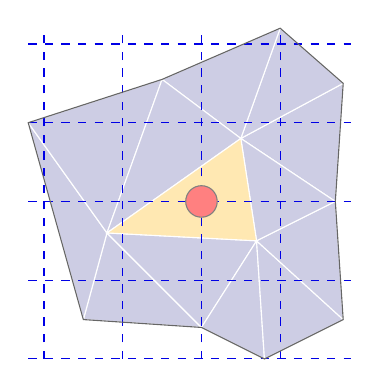
\begin{tikzpicture}
		%---Interno---
	%1 - (-1.2, -0.4)
	\draw[white, fill=blue!30!gray!30!white] (-1.5, -1.5) -- (0,-1.6) -- (-1.2, -0.4) -- cycle;
	\draw[white, fill=blue!30!gray!30!white] (-2.2, 1) -- (-1.5,-1.5) -- (-1.2, -0.4) -- cycle;
	\draw[white, fill=blue!30!gray!30!white] (-2.2, 1) -- (-0.5, 1.55) -- (-1.2, -0.4) -- cycle;
	%2 - (0.7, -0.5)
	\draw[white, fill=blue!30!gray!30!white] (-1.2, -0.4) -- (0,-1.6) -- (0.7, -0.5) -- cycle;
	\draw[white, fill=blue!30!gray!30!white] (0.8,-2) -- (0,-1.6) -- (0.7, -0.5) -- cycle;
	\draw[white, fill=blue!30!gray!30!white] (1.8,-1.5) -- (0.8,-2) -- (0.7, -0.5) -- cycle;
	\draw[white, fill=blue!30!gray!30!white] (1.8,-1.5) -- (1.7,0) -- (0.7, -0.5) -- cycle;
	%3 - (0.5,0.8)
	\draw[white, fill=blue!30!gray!30!white] (1.7,0) -- (1.8,1.5) -- (0.5, 0.8) -- cycle;
	\draw[white, fill=blue!30!gray!30!white] (1.7,0) -- (0.7, -0.5) -- (0.5, 0.8) -- cycle;
	\draw[white, fill=blue!30!gray!30!white] (1,2.2) -- (1.8,1.5) -- (0.5, 0.8) -- cycle;
	\draw[white, fill=blue!30!gray!30!white] (-0.5,1.55) -- (1,2.2) -- (0.5, 0.8) -- cycle;
	\draw[white, fill=blue!30!gray!30!white] (-1.2,-0.4) -- (-0.5,1.55) -- (0.5, 0.8) -- cycle;
	\draw[white, fill=red!30!yellow!30!white] (-1.2,-0.4) -- (0.7,-0.5) -- (0.5, 0.8) -- cycle;
	
	%malla
	\draw[step=1, dashed, blue!90!black] (-2.2, -2) grid (1.9,2.2);
	
	%Partículas
	\draw[black!50, fill=red!50] (0,0) circle (2mm);
	
	%Carcasa
	\draw[black!60] (-2.2, 1) -- (-0.5, 1.55) -- (1, 2.2) -- (1.8, 1.5) -- (1.7, 0) -- (1.8, -1.5) -- (0.8, -2) -- (0, -1.6) -- (-1.5, -1.5) -- cycle;
	 
		\end{tikzpicture}
		\end{adjustbox}
	\caption{Mapeo de una part\'icula dada dentro del fluido para interpolar sus propiedades en ese punto.}
	\end{subfigure}
	\hfill
	\begin{subfigure}[b]{0.3\textwidth}
		\centering
		\begin{adjustbox}{max width = \textwidth}
		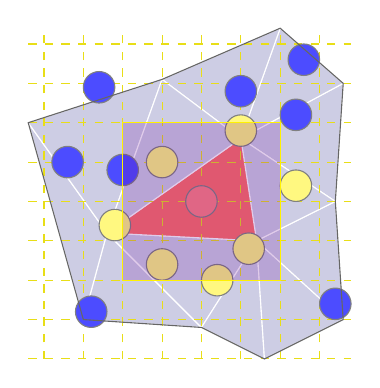
\begin{tikzpicture}
		%---Interno---
	%1 - (-1.2, -0.4)
	\draw[white, fill=blue!30!gray!30!white] (-1.5, -1.5) -- (0,-1.6) -- (-1.2, -0.4) -- cycle;
	\draw[white, fill=blue!30!gray!30!white] (-2.2, 1) -- (-1.5,-1.5) -- (-1.2, -0.4) -- cycle;
	\draw[white, fill=blue!30!gray!30!white] (-2.2, 1) -- (-0.5, 1.55) -- (-1.2, -0.4) -- cycle;
	%2 - (0.7, -0.5)
	\draw[white, fill=blue!30!gray!30!white] (-1.2, -0.4) -- (0,-1.6) -- (0.7, -0.5) -- cycle;
	\draw[white, fill=blue!30!gray!30!white] (0.8,-2) -- (0,-1.6) -- (0.7, -0.5) -- cycle;
	\draw[white, fill=blue!30!gray!30!white] (1.8,-1.5) -- (0.8,-2) -- (0.7, -0.5) -- cycle;
	\draw[white, fill=blue!30!gray!30!white] (1.8,-1.5) -- (1.7,0) -- (0.7, -0.5) -- cycle;
	%3 - (0.5,0.8)
	\draw[white, fill=blue!30!gray!30!white] (1.7,0) -- (1.8,1.5) -- (0.5, 0.8) -- cycle;
	\draw[white, fill=blue!30!gray!30!white] (1.7,0) -- (0.7, -0.5) -- (0.5, 0.8) -- cycle;
	\draw[white, fill=blue!30!gray!30!white] (1,2.2) -- (1.8,1.5) -- (0.5, 0.8) -- cycle;
	\draw[white, fill=blue!30!gray!30!white] (-0.5,1.55) -- (1,2.2) -- (0.5, 0.8) -- cycle;
	\draw[white, fill=red!95!yellow!60!white] (-1.2,-0.4) -- (0.7,-0.5) -- (0.5, 0.8) -- cycle;
	\draw[white, fill=blue!30!gray!30!white] (-1.2,-0.4) -- (-0.5,1.55) -- (0.5, 0.8) -- cycle;
	
	%malla
	\draw[step=0.5, dashed, yellow!90!black] (-2.2, -2) grid (1.9,2.2);
	
	%Partículas
	\draw[black!50, fill=red!50] (0,0) circle (2mm);
	\draw[black!50, fill=yellow!50] (0.6,-0.6) circle (2mm);
	\draw[black!50, fill=yellow!50] (-1.1,-0.3) circle (2mm);
	\draw[black!50, fill=yellow!50] (0.5,0.9) circle (2mm);
	\draw[black!50, fill=yellow!50] (-0.5,0.5) circle (2mm);
	\draw[black!50, fill=yellow!50] (1.2,0.2) circle (2mm);
	\draw[black!50, fill=yellow!50] (-0.5,-0.8) circle (2mm);
	\draw[black!50, fill=yellow!50] (0.2,-1) circle (2mm);
	
	\draw[black!50, fill=blue!70] (1.7,-1.3) circle (2mm);
	\draw[black!50, fill=blue!70] (-1.4,-1.4) circle (2mm);
	\draw[black!50, fill=blue!70] (-1,0.4) circle (2mm);
	\draw[black!50, fill=blue!70] (-1.7, 0.5) circle (2mm);
	\draw[black!50, fill=blue!70] (-1.3,1.45) circle (2mm);
	\draw[black!50, fill=blue!70] (1.2, 1.1) circle (2mm);
	\draw[black!50, fill=blue!70] (0.5,1.4) circle (2mm);
	\draw[black!50, fill=blue!70] (1.3,1.8) circle (2mm);
	
	%Carcasa
	\draw[black!60] (-2.2, 1) -- (-0.5, 1.55) -- (1, 2.2) -- (1.8, 1.5) -- (1.7, 0) -- (1.8, -1.5) -- (0.8, -2) -- (0, -1.6) -- (-1.5, -1.5) -- cycle;
	
	\draw[yellow, fill=red!40!blue, fill opacity=0.2] (-1,-1) rectangle (1,1);
		\end{tikzpicture}
		\end{adjustbox}
	\caption{Mapeo del elemento de malla CFD para el c\'alculo de t\'erminos fuente en el elemento de inter\'es.}
	\end{subfigure}
	\caption{Esquema de la aproximaci\'on por malla dual para la b\'usqueda de part\'iculas vecinas en un fluido.}
	\label{particle}
\end{figure}

\noindent
\justify

Los pasos clave con los que se basan las mallas de b\'usqueda son: detecci\'on de colisi\'on de part\'iculas (descrito en la secci\'on \ref{detect}), geometr\'ia de los elementos de malla CFD (detallado en la secci\'on \ref{CFD2D}) y el c\'alculo de fuerzas de fluido, entre otras.

\noindent
\justify

Para el c\'alculo de las fuerzas ejercidas por el fluido, se requiere conocer las propiedades del fluido en la posici\'on de la part\'icula; incluyendo el gradiente de presi\'on, la velocidad del flujo y el gradiente de velocidades (para fluidos gaseosos). Normalmente, las propiedades del fluido se `almacenan' en el centroide de los elementos de malla durante c\'alculos mediante FVM, como se muestra en la Ecuaci\'on \ref{properties}.

\begin{equation}
\phi _p = \phi _{el} + \nabla \phi _{el} \cdot r_{pc}
\label{properties}
\end{equation}

\noindent
\justify

D\'onde: $\phi _p$ y $\phi _{el}$ son las propiedades del fluido en la posici\'on de la part\'icula y el centroide del elemento, respectivamente; y $r_{pc}$ es el vector distancia que va desde el centro del elemento hasta la posici\'on de la part\'icula. 

\subsubsection{Enfoque \textit{Eulerian - Lagrange}} \label{EuLag}

\noindent
\justify

La tasa de part\'iculas debido a la sedimentaci\'on, a trav\'es de canales inclinados, ha sido ampliamente estudiado debido al reconocido \textit{efecto Boycott}$^{\cite{Xu2005}}$. Este fen\'omeno se produce por el incremento en el \'area efectiva de sedimentaci\'on debido a la presencia de placas inclinadas$^{\cite{Galvin2002}}$. Acrivos $^{\cite{Acrivos1995}}$ desarroll\'o una serie de planteamientos te\'oricos y experimentales entre la tasa de sedimentaci\'on de part\'iculas y el \'area efectiva de sedimentaci\'on. El efecto Boycott ha sido aplicado con \'exito en diversos procesos industriales para la remoci\'on de part\'iculas en lecho de fluidizado a trav\'es del asentamiento gravitacional; entre los principales ejemplos de este hecho se encuentran: tratamientos de aguas residuales y procesos de filtrado de agua.

\noindent
\justify

El acercamiento experimental para la investigaci\'on caracter\'istica de part\'iculas en suspenci\'on a alta concentraci\'on ha demostrado ser una experiencia retadora debido a las limitantes instrumentales y t\'ecnicas de medici\'on$^{\cite{Galvin2002}}$. Los modelos num\'ericos basados en CFD han demostrado ser una herramienta poderosa y promisoria que provee informaci\'on detallada y precisa sobre las caracter\'isticas locales del flujo particulado. Normalmente, se han aplicado dos enfoques generales en la literatura para resolver problemas que involucran flujo particulado: \textit{Eulerian - Eulerian} (E-E) y \textit{Eulerian - Lagrange} (E-L). En el enfoque E-E, las fases s\'olida y fluida son interpretadas de manera continua en donde comparten el mismo grupo de ecuaciones gobernantes. Doroodchi \textit{et al.}$^{\cite{Doroodchi2005}}$ emplearon el modelo E-E para investigar la influencia de las placas inclinadas y el efecto expansivo de s\'olidos en suspensi\'on en camas de lecho fluidizado; obteniendo resultados prometedores tanto en la parte experimental como num\'erica. Salem \textit{et al} $^{\cite{Salem2011}}$ desarrollaron un modelamiento en CFD empleando el modelo E-E para evaluar las caracter\'isticas hidr\'aulicas de un sedimentador de placas hidr\'aulicas (IPS, por sus siglas en ingl\'es); demostrando el importante rol que cumplen las herramientas computacionales en el estudio de los sistemas de sedimentaci\'on. Sin embargo, el tratamiento de la fase s\'olida de manera continua va en contra de la naturaleza discreta de las part\'iculas s\'olidas, y todav\'ia m\'as importante: el acercamiento a trav\'es de E-E carece de facultades num\'ericas para revelar informaci\'on importante referente a la escala particular.

\noindent
\justify

El enfoque otorgado por el modelo E-L, por otro lado, adopta la teor\'ia continua para la fase l\'iquida y resuelve el problema cinem\'atico de cada part\'icula individual \textbf{directamente}. Informaci\'on referente a la posici\'on, velocidad, fuerza hidrodin\'amica y difusividad, entre otros, se pueden obtener para cualquier instante de tiempo. Teniendo as\'i el potencial de sobrellevar las dificultades y limitaciones existentes en modelos te\'oricos y emp\'iricos. Es debido a ello que en el \textit{presente trabajo} se emplea un enfoque E-L para abordar el problema CFD-DEM; investigando la interacci\'on fluido - part\'icula en un sistema de sedimentaci\'on con canales (lamelas) inclinadas.

\paragraph{Planteamiento num\'erico}

\noindent
\justify

El flujo del modelo CFD-DEM se resuelve a trav\'es de las ecuaciones de momento, continuidad y a trav\'es de las ecuaciones de movimiento de cada part\'icula individual, seguidas a trav\'es del m\'etodo de elementos discretos$^{\cite{Peng2014}}$. Se consideraron los efectos e interacciones entre part\'icula-part\'icula (ver Figura \ref{particula}), part\'icula-fluido y part\'icula-muro. Las ecuaciones gobernantes y la metodolog\'ia num\'erica empleada se describe brevemente a continuaci\'on.

\begin{figure}[h!]
	\centering
	\begin{subfigure}[b]{0.4\textwidth}
		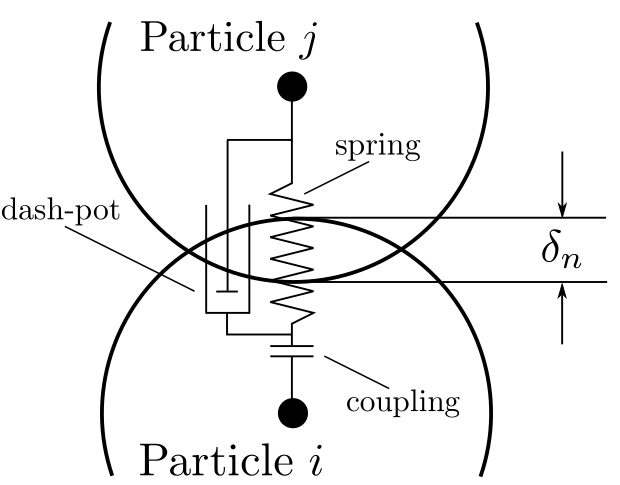
\includegraphics[width=\textwidth]{Images/normal.png}
		\caption{Fuerza normal.}
	\end{subfigure}
	\hfill
	\begin{subfigure}[b]{0.4\textwidth}
		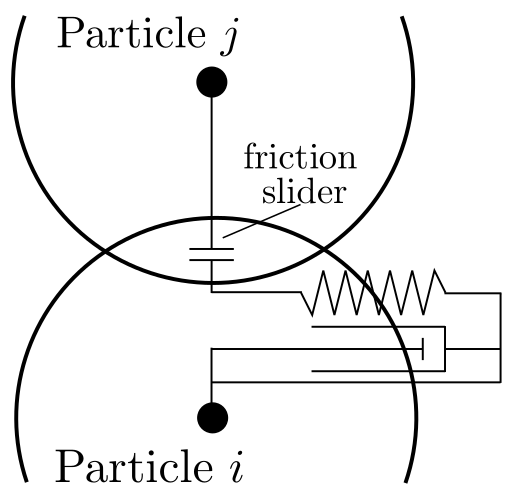
\includegraphics[width=0.8\textwidth]{Images/tangencial.png}
		\caption{Fuerza tangencial.}
	\end{subfigure}
	\caption{Interacci\'on din\'amica entre part\'iculas.}
	\label{particula}
\end{figure}

\noindent
\justify

En DEM, no se requiere de un \textit{cierre} para la fase s\'olida dado que la din\'amica de la part\'icula se resuelve de manera directa. La traslaci\'on y rotaci\'on de la part\'icula $i$ est\'a dada por las Ecuaciones \ref{DEMdyn} y \ref{DEMrot}.

\begin{equation}
	m_i \frac{d v _i}{dt} = F_{c,i} + F_{f,i} + F_{g,i}
	\label{DEMdyn}
\end{equation}

\begin{equation}
	I_i \frac{d \omega _i}{dt} = T_{c,i} + T_{r,i}
	\label{DEMrot}
\end{equation}

\noindent
\justify

Las fuerzas de impacto $\left( F_{c,i} \right)$ y el torque de contacto $\left( T_{c,i} \right)$ fueron calculados por el modelo lineal resorte-dashpot en el que se tuvo en cuenta el efecto hister\'etico causado por el historial de contacto de la part\'icula. La resistencia a la rodadura se calcul\'o empleando la Ecuaci\'on \ref{rolling}.

\begin{equation}
	T_{r,i} = - \sum _{j=0} ^{N_{pc}} \mu _{rol}  \left|F_{cn, ij} \right| \frac{\omega _{ij}}{\left| \omega _{ij} \right|} r_i
	\label{rolling}
\end{equation}

\noindent
\justify

D\'onde $\omega _{ij}$ es la velocidad angular relativa entre las part\'iculas $i$ y $j$; y est\'a definida a trav\'es de la Ecuaci\'on \ref{omega}.

\begin{equation}
	\omega _{ij} = \frac{\omega _i r_i + \omega _j r_j}{r_i + r_j}
	\label{omega}
\end{equation}

\noindent
\justify

La fuerza total actuante del fluido $F_{f,i}$ causada por la distorsi\'on de las l\'ineas de corriente alrededor de la part\'icula, que a su vez produce variaci\'on en el tensor de esfuerzos del fluido, se calcula mediante la Ecuaci\'on \ref{ffi}.

\begin{equation}
	F_{f,i} = - V_i \nabla p + V_i \left( \nabla \cdot \tau _f \right) + \epsilon F_{d,i}
	\label{ffi}
\end{equation}

\noindent
\justify

D\'onde $\tau _f$ es el tensor de esfuerzos viscoso del fluido; que se calcula de la siguiente manera:

\begin{equation}
	\tau _f = \mu _L \left[ \left( \nabla u_L \right) + \left( \nabla u_L \right) ^{-1} \right] + \left(\lambda - \frac{2}{3} \mu \right) \left( \nabla \cdot u_L \right) \overline{I}
\end{equation}

\noindent
\justify

La fuerza de arrastre $F_{d,i}$ del fluido, de la Ecuaci\'on \ref{ffi}, se resuelve a una escala longitudinal mayor que el tama\~no de la part\'icula y est\'a dada por la siguiente relaci\'on matem\'atica:

\begin{equation}
	F_{d,i} = \frac{V_i}{1 - \epsilon} \beta \left( u_L - v_i \right)
\end{equation}